\documentclass[english,reprint, aps, prl,superscriptaddress, showpacs,
showkeys, longbibliography, amsmath, amssymb, floatfix]{revtex4-1} 
\pdfoutput=1

\usepackage{fullpage}
\usepackage{cmap}
\usepackage[T1,T2A]{fontenc}
\usepackage[utf8]{inputenc}
\usepackage[french,main=english]{babel}
\usepackage{amsthm}
\usepackage{mathrsfs}
\usepackage{bbold}
\usepackage{wesa}
\usepackage{graphicx}
\usepackage{verbatim}
\usepackage[backref=false]{hyperref}
\usepackage{booktabs}
\usepackage{multirow}
\usepackage[braket,qm]{qcircuit}
\usepackage{color}
\usepackage[usenames,dvipsnames]{xcolor}
\usepackage{framed}
\usepackage{comment}
\usepackage{xparse}

\theoremstyle{plain}
\newtheorem{thm}{Theorem}
\newtheorem{lemma}{Lemma}[thm]
\newtheorem{cor}{Corollary}[thm]
\newtheorem{assumption}{Assumption}
\newtheorem{fact}{Fact}
\theoremstyle{definition}
\newtheorem{definition}{Definition}
\newtheorem{condition}[assumption]{Condition}

\DeclareUnicodeCharacter{0229}{\c{e}}

\newcommand{\Hilb}{\mathcal{H}}
\newcommand{\events}{\ensuremath{\mathcal{E}}}
\newcommand{\qevents}{\ensuremath{\mathcal{E}}}
\newcommand{\pmeas}{\ensuremath{\mu}}
% \newcommand{\imposs}{{\text{\wesa{impossible}}}}
% \newcommand{\likely}{{\text{\wesa{likely}}}}
% \newcommand{\unlikely}{{\text{\wesa{unlikely}}}}
% \newcommand{\necess}{{\text{\wesa{certain}}}}
% \newcommand{\unknown}{{\text{\wesa{unknown}}}}
% \newcommand{\midd}{{\text{\wesa{middle}}}}
\newcommand{\imposs}{\ensuremath{\left[0,0\right]}}
\newcommand{\likely}{\ensuremath{\left[\tfrac{1}{2},1\right]}}
\newcommand{\unlikely}{\ensuremath{\left[0,\tfrac{1}{2}\right]}}
\newcommand{\necess}{\ensuremath{\left[1,1\right]}}
\newcommand{\unknown}{\ensuremath{\left[0,1\right]}}
\newcommand{\midd}{\ensuremath{\left[\tfrac{1}{4},\tfrac{3}{4}\right]}}
\newcommand{\fket}[1]{{|#1\rangle}}
\newcommand{\fproj}[1]{|#1\rangle\langle #1|}
\newcommand{\proj}[1]{\op{#1}{#1}}
\newcommand{\ps}{\texttt{+}}
\newcommand{\ms}{\texttt{-}}
\newcommand{\set}[2]{\ensuremath{\left\{ {#1}\mathrel{}\middle|\mathrel{}{#2}\right\} }}
\newcommand{\Tr}{\ensuremath{\mathop{\mathrm{Tr}}\nolimits}}
\allowdisplaybreaks
\newcommand{\coreBorn}{\ensuremath{\overline{\Hilb}}}
\newcommand{\mul}[1][]{\ensuremath{\mu^{L{#1}}}}
\newcommand{\mur}[1][]{\ensuremath{\mu^{R{#1}}}}
\setcounter{secnumdepth}{3}
% https://tex.stackexchange.com/questions/345284/can-i-have-an-almost-non-breaking-space-in-latex
% Change non-breaking space to \nolinebreak[1] 
% Hence, it will not hyphenate too much surrounding words.
\newcommand{\rmd}{d}
\newcommand{\rmi}{i}
\lineskiplimit=1pt
\newcommand{\ultramodular}{\mathcal{M}}
\newcommand{\ultramodularL}[1][]{\ensuremath{\ultramodular^{L{#1}}}}
\newcommand{\ultramodularR}[1][]{\ensuremath{\ultramodular^{R{#1}}}}
\newcommand{\muB}{\ensuremath{\mu^{B}}}
\newcommand{\eventsC}{\ensuremath{\events_{C}}}

\newcommand{\says}[3]{\begin{framed}\begin{minipage}{0.9\linewidth}\color{#1}{#2 says: #3}\end{minipage}\end{framed}}
\newcommand{\amr}[1]{\says{green}{Amr}{#1}}
\newcommand{\yutsung}[1]{\says{purple}{Yu-Tsung}{#1}}
\newcommand{\gerardo}[1]{\says{OliveGreen}{Gerardo}{#1}}
\newcommand{\andy}[1]{\says{blue}{Andy}{#1}}
% \excludecomment{suggest}
\NewDocumentEnvironment{suggest}{m m O{}}{#1{TEXT \##2 would go here. #3}}{#1{TEXT \##2 end here.}}

\newcommand{\happen}{\text{H}}
\newcommand{\notHappen}{\text{N}}
\newcommand{\missing}{\text{M}}
%%%%%%%%%%%%%%%%%%%%%%%%%%%%%%%%%%%%%%%%%%%%%%%%%%%%%%%%%%%%%%%%%%%
\begin{document}

\title{Response to the Referee Report of ``Quantum Interval-Valued Probability:
Contextuality and the Born Rule''}

\author{Yu-Tsung Tai}

\affiliation{Department of Mathematics, Indiana University, Bloomington, Indiana
47405, USA}

\affiliation{Department of Computer Science, Indiana University, Bloomington,
Indiana 47405, USA}

\author{Andrew J. Hanson}

\affiliation{Department of Informatics, Indiana University, Bloomington, Indiana
47405, USA}

\author{Gerardo Ortiz}

\affiliation{Department of Physics, Indiana University, Bloomington, Indiana 47405,
USA}

\author{Amr Sabry}

\affiliation{Department of Computer Science, Indiana University, Bloomington,
Indiana 47405, USA}

\date{\today}

\maketitle
%%%%%%%%%%%%%%%%%%%%%%%%%%%%%%%%%%%%%%%%%%%%%%%%%%%%%%%%%%%%%%%%%%%

\section{Why a \texorpdfstring{$\frac{1}{4}$}{¼}-deterministic QIVPM is
Impossible?}

To illustrate our proof for non-existence of $\delta$-deterministic
QIVPMs for $\delta<\frac{1}{3}$, we will explain why we cannot construct
any $\frac{1}{4}$-deterministic QIVPM in full details. The proof
is by contradiction: Suppose there is a $\frac{1}{4}$-deterministic
QIVPM~$\bar{\mu}:\events\rightarrow\mathscr{I}$. Now use this assumed
QIVPM to construct the following $0$-deterministic QIVPM $\bar{\mu}^{\textrm{D}}:\events\rightarrow\left\{ \imposs,\necess\right\} $:
\begin{equation}
\bar{\mu}^{\textrm{D}}\left(P\right)=\begin{cases}
\imposs\,, & \textrm{ if }\bar{\mu}\left(P\right)\subseteq\left[0,\tfrac{1}{4}\right]\:;\\
\necess\,, & \textrm{ if }\bar{\mu}\left(P\right)\subseteq\left[\tfrac{3}{4},1\right]\:.
\end{cases}
\end{equation}
However, since we know that $0$-deterministic QIVPMs do not exist~\cite{THOS2017},
the map $\bar{\mu}^{\textrm{D}}$ cannot exist and hence $\bar{\mu}$
does not exist. It remains to verify that $\bar{\mu}^{\textrm{D}}$
is indeed a QIVPM by checking that for orthogonal projectors $P_{0}$
and~$P_{1}$, 
\begin{equation}
\bar{\mu}^{\textrm{D}}\left(P_{0}+P_{1}\right)=\bar{\mu}^{\textrm{D}}\left(P_{0}\right)+\bar{\mu}^{\textrm{D}}\left(P_{1}\right)\,,\label{eq:QuantumInterval-valuedProbability-Equal}
\end{equation}
because similar to classical inclusion-exclusion principle, Eq.~(\ref{eq:QuantumInterval-valuedProbability-Equal})
implies for each pair of commuting projectors $P_{0}$ and~$P_{1}$,
\begin{equation}
\begin{aligned} & \bar{\mu}^{\textrm{D}}\left(P_{0}+P_{1}-P_{0}P_{1}\right)+\bar{\mu}^{\textrm{D}}\left(P_{0}P_{1}\right)\\
={} & \bar{\mu}^{\textrm{D}}\left(P_{0}\right)+\bar{\mu}^{\textrm{D}}\left(P_{1}\right)\,,
\end{aligned}
\end{equation}
i.e., $\bar{\mu}^{\textrm{D}}$ is convex.

For orthogonal projectors~$P_{0}$ and $P_{1}$, when one of $\bar{\mu}^{\textrm{D}}\left(P_{0}\right)$
and $\bar{\mu}^{\textrm{D}}\left(P_{1}\right)$ is $\necess$, say
$\bar{\mu}^{\textrm{D}}\left(P_{0}\right)=\necess$. Then, $\bar{\mu}^{\textrm{D}}\left(P_{1}\right)=\imposs$
and 
\begin{equation}
\begin{aligned} & \bar{\mu}\left(P_{0}+P_{1}\right)\subseteq\bar{\mu}\left(P_{0}\right)+\bar{\mu}\left(P_{1}\right)\\
\subseteq{} & \left[\tfrac{3}{4},1\right]+\left[0,\tfrac{1}{4}\right]=\left[\tfrac{3}{4},\tfrac{5}{4}\right]\,.
\end{aligned}
\end{equation}
Since $\bar{\mu}\left(P_{0}+P_{1}\right)$ is bounded by $\left[0,1\right]$,
we must have $\bar{\mu}\left(P_{0}+P_{1}\right)\subseteq\left[\frac{3}{4},1\right]$,
i.e., $\bar{\mu}^{\textrm{D}}\left(P_{0}+P_{1}\right)=\necess=\bar{\mu}^{\textrm{D}}\left(P_{0}\right)+\bar{\mu}^{\textrm{D}}\left(P_{1}\right)$.

\begin{figure*}
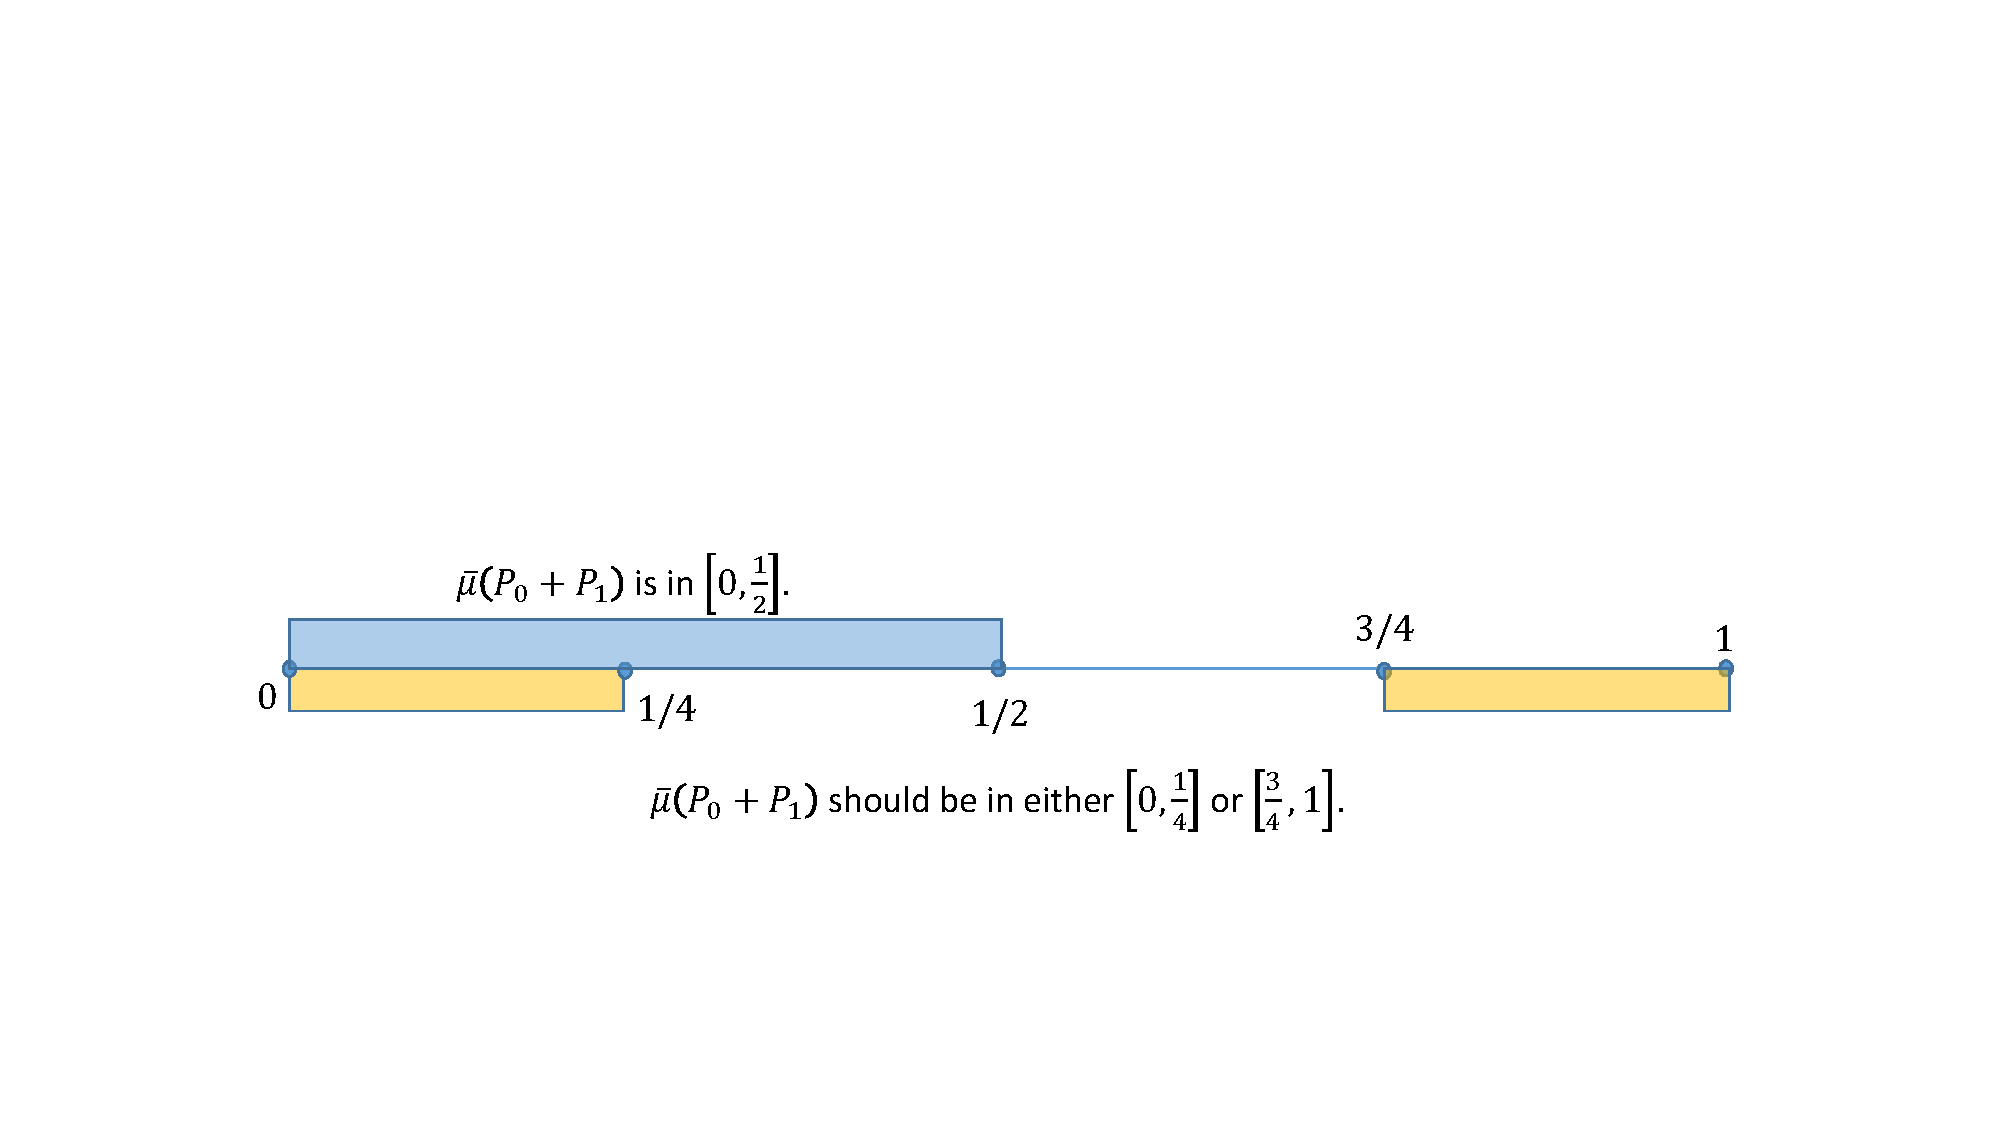
\includegraphics[bb=50bp 100bp 900bp 300bp,clip,scale=0.5]{prop_prop_letter_ajhs_referee_response_pptx}\caption{\label{fig:Show-subset}Show $\bar{\mu}\left(P_{0}+P_{1}\right)$
must be a subset of $\left[0,\frac{1}{4}\right]$.}
\end{figure*}
For orthogonal projectors~$P_{0}$ and $P_{1}$, when $\bar{\mu}^{\textrm{D}}\left(P_{0}\right)=\bar{\mu}^{\textrm{D}}\left(P_{1}\right)=\imposs$,
we have both $\bar{\mu}\left(P_{0}\right)$ and $\bar{\mu}\left(P_{1}\right)\subseteq\left[0,\frac{1}{4}\right]$
which implies $\bar{\mu}\left(P_{0}+P_{1}\right)\subseteq\left[0,\frac{1}{2}\right]$.
Since $\bar{\mu}\left(P_{0}+P_{1}\right)$ is a subset of either $\left[0,\frac{1}{4}\right]$
or $\left[\tfrac{3}{4},1\right]$ and the latter is excluded as illustrated
in Fig.~\ref{fig:Show-subset} , then $\bar{\mu}\left(P_{0}+P_{1}\right)$
must be a subset of $\left[0,\frac{1}{4}\right]$, which implies $\bar{\mu}^{\textrm{D}}\left(P_{0}+P_{1}\right)=\imposs$.

After we explained why there is no $\delta$-deterministic QIVPMs
for $\delta<\frac{1}{3}$, we are going to explain the physical meaning
of $\delta$-deterministic, and understand the transition from $\delta<\frac{1}{3}$
to $\delta\ge\frac{1}{3}$.

\section{Physical Meaning of $\delta$-Determinism}

Since QIVPMs are extensional of both quantum probability measures
and classical IVPMs, the meaning of $\delta$-determinism can be explained
better when we consider $\delta$-deterministic classical IVPMs.

\begin{definition}[$\delta$-Determinism for classical IVPMs]\label{def:delta-deterministic-classical}
Given a classical IVPM~$\bar{\mu}:\eventsC\rightarrow\mathscr{I}$,
where $\eventsC$ is the set of mutually commuting events. Then, $\bar{\mu}$
is $\delta$-deterministic if, for every event $P\in\events'$, we
have either $\bar{\mu}\left(P\right)\subseteq\left[0,\delta\right]$
or $\bar{\mu}\left(P\right)\subseteq\left[1-\delta,1\right]$. \end{definition}

\begin{table}
\noindent \centering{}\caption{\label{tab:classical-IVPMs}Examples of $\delta$-deterministic classical
IVPMs $\bar{\mu}_{A}$ and $\bar{\mu}_{B}$ on commuting events $P$.}
\begin{tabular}{ccc}
\toprule 
\addlinespace
$P$  & $\bar{\mu}_{A}(P)$  & $\bar{\mu}_{B}(P)$ \tabularnewline
\midrule
\midrule 
\addlinespace
$\mathbb{0}$  & $\imposs$  & $\imposs$ \tabularnewline
\midrule 
\addlinespace
$\proj{0}$  & $\necess$  & $\left[\frac{3}{4},\frac{4}{5}\right]$ \tabularnewline
\midrule 
\addlinespace
$\proj{1}$  & $\imposs$  & $\left[\frac{1}{5},\frac{1}{4}\right]$ \tabularnewline
\midrule 
\addlinespace
$\mathbb{1}$  & $\necess$  & $\necess$ \tabularnewline
\bottomrule
\end{tabular}
\end{table}

\noindent It is easy to construct $\delta$-deterministic classical
IVPMs $\bar{\mu}_{A}$ and $\bar{\mu}_{B}$ defined in Table~\ref{tab:classical-IVPMs},
where $\proj{0}$ and $\proj{1}$ represents heads and tails in coin-tossing,
respectively. The interpretation for $\bar{\mu}_{A}$ is that we have
a double-headed coin that always comes up heads. For $\bar{\mu}_{B}$,
the interpretation is that we throw a coin $1000$ times and we observe
$750$ heads and $200$ tails and the coin falls under the couch $50$
times. For $\bar{\mu}_{A}$, $\delta$ is $0$; for $\bar{\mu}_{B}$,
$\delta=\frac{1}{4}$, and $\delta$ qualifies how close a coin is
to double-headed (or double-tailed), which we can certainly know the
outcome of a coin even before tossing. We see here that we can construct
$0$-deterministic as well as $\frac{1}{4}$-deterministic and in
fact for any $\delta$ in the range $\left[0,1\right]$ we can construct
a $\delta$-deterministic classical probability measure. BUT the situation
changes in the quantum case, WE CANNOT construct $\delta$-deterministic
probability measures for $\delta<\frac{1}{3}$.

\section{Why a \texorpdfstring{$\frac{1}{3}$}{⅓}-deterministic QIVPM exists?}

\begin{table}
\noindent \centering{}\caption{\label{tab:classical-IVPMs-results}A sample experimental record for
a classical experiment with three possible outcomes $\proj{0}$, $\proj{1}$,
and $\proj{2}$. A event can be happened ($\happen$) or not happened
($\notHappen$), and the experimental results could be summarized
by a $0$-deterministic classical IVPM~$\bar{\mu}_{\ref{tab:classical-IVPMs-results}}$.}
\begin{tabular}{ccccc}
\toprule 
\addlinespace
$P$  & Trial~0 & Trial~1 & Trial~2 & $\bar{\mu}_{\ref{tab:classical-IVPMs-results}}(P)$\tabularnewline
\midrule
\midrule 
\addlinespace
$\mathbb{0}$  & $\notHappen$ & $\notHappen$ & $\notHappen$ & $\imposs$\tabularnewline
\midrule 
\addlinespace
$\proj{0}$  & $\notHappen$ & $\notHappen$ & $\notHappen$ & $\imposs$\tabularnewline
\midrule 
\addlinespace
$\proj{1}$  & $\notHappen$ & $\notHappen$ & $\notHappen$ & $\imposs$\tabularnewline
\midrule 
\addlinespace
$\proj{2}$ & $\happen$ & $\happen$ & $\happen$ & $\necess$\tabularnewline
\midrule 
\addlinespace
$\mathbb{1}-\proj{0}$  & $\happen$ & $\happen$ & $\happen$ & $\necess$\tabularnewline
\midrule 
\addlinespace
$\mathbb{1}-\proj{1}$  & $\happen$ & $\happen$ & $\happen$ & $\necess$\tabularnewline
\midrule 
\addlinespace
$\mathbb{1}-\proj{2}$ & $\notHappen$ & $\notHappen$ & $\notHappen$ & $\imposs$\tabularnewline
\midrule 
\addlinespace
$\mathbb{1}$  & $\happen$ & $\happen$ & $\happen$ & $\necess$\tabularnewline
\bottomrule
\end{tabular}
\end{table}
Sample experimental results with three possible outcomes $\proj{0}$,
$\proj{1}$, and $\proj{2}$ are listed in Table~\ref{tab:classical-IVPMs-results}.
Because the results of every event are always the same, they could
be summarized to a $0$-deterministic classical IVPM~$\bar{\mu}_{\ref{tab:classical-IVPMs-results}}$.
Given any Hilbert space of dimension~$d\ge3$, the Kochen-Specker
theorem asserts that we cannot have a table where every event always
has the same result~\cite{THOS2017}. 
\begin{table}
\noindent \centering{}\caption{\label{tab:quantum-IVPMs-results}A sample inconsistent experimental
record for a quantum experiment on a three-dimensional Hilbert space,
where $\proj{\psi}$ is any one-dimensional projector, and $\mathbb{1}-\proj{\psi}$
is any two-dimensional projector. A event can be happened ($\happen$)
or not happened ($\notHappen$), but $\bar{\mu}_{\ref{tab:quantum-IVPMs-results}}$
that summarizes the experimental results is not a QIVPM.}
\begin{tabular}{ccccc}
\toprule 
\addlinespace
$P$  & Trial~0 & Trial~1 & Trial~2 & $\bar{\mu}_{\ref{tab:quantum-IVPMs-results}}(P)$\tabularnewline
\midrule
\midrule 
\addlinespace
$\mathbb{0}$  & $\notHappen$ & $\notHappen$ & $\notHappen$ & $\imposs$\tabularnewline
\midrule 
\addlinespace
$\proj{\psi}$  & $\notHappen$ & $\notHappen$ & $\notHappen$ & $\imposs$\tabularnewline
\midrule 
\addlinespace
$\mathbb{1}-\proj{\psi}$  & $\happen$ & $\happen$ & $\happen$ & $\necess$\tabularnewline
\midrule 
\addlinespace
$\mathbb{1}$  & $\happen$ & $\happen$ & $\happen$ & $\necess$\tabularnewline
\bottomrule
\end{tabular}
\end{table}
For example, Table~\ref{tab:quantum-IVPMs-results} doesn't give
coherent experimental results, and cannot be summarized as a QIVPM
because given any two distinct one-dimensional projectors $P_{0}$
and $P_{1}$, 
\begin{equation}
\begin{aligned} & \bar{\mu}_{\ref{tab:quantum-IVPMs-results}}\left(P_{0}+P_{1}-P_{0}P_{1}\right)+\bar{\mu}_{\ref{tab:quantum-IVPMs-results}}\left(P_{0}P_{1}\right)=\necess\\
\nsubseteq{} & \imposs=\bar{\mu}_{\ref{tab:quantum-IVPMs-results}}\left(P_{0}\right)+\bar{\mu}_{\ref{tab:quantum-IVPMs-results}}\left(P_{1}\right)\,.
\end{aligned}
\end{equation}

\begin{table}
\noindent \centering{}\caption{\label{tab:quantum-IVPMs-missing}A sample experimental record for
a quantum experiment on a three-dimensional Hilbert space with some
records missing. Now a event can be happened ($\happen$), not happened
($\notHappen$), or missing ($\missing$), and $\proj{\psi_{i}}$
is any one-dimensional projector with Trial~$i$ missing, and $\mathbb{1}-\proj{\psi_{i}}$
is any two-dimensional projector with Trial~$i$ missing. Although
$\bar{\mu}_{\ref{tab:quantum-IVPMs-missing}}$ which summarizes the
experimental results is not directly a QIVPM, the whole records might
come from coherent experimental results with a QIVPM $\bar{\mu}_{\ref{tab:quantum-IVPMs-missing}}'$.}
\begin{tabular}{cccccc}
\toprule 
\addlinespace
$P$  & Trial~0 & Trial~1 & Trial~2 & $\bar{\mu}_{\ref{tab:quantum-IVPMs-missing}}(P)$ & $\bar{\mu}_{\ref{tab:quantum-IVPMs-missing}}'(P)$\tabularnewline
\midrule
\midrule 
\addlinespace
$\mathbb{0}$  & $\notHappen$ & $\notHappen$ & $\notHappen$ & $\imposs$ & $\imposs$\tabularnewline
\midrule 
\addlinespace
$\proj{\psi_{0}}$  & $\missing$ & $\notHappen$ & $\notHappen$ & $\left[0,\frac{1}{3}\right]$ & $\left[\frac{1}{3},\frac{1}{3}\right]$\tabularnewline
\midrule 
\addlinespace
$\proj{\psi_{1}}$  & $\notHappen$ & $\missing$ & $\notHappen$ & $\left[0,\frac{1}{3}\right]$ & $\left[\frac{1}{3},\frac{1}{3}\right]$\tabularnewline
\midrule 
\addlinespace
$\proj{\psi_{2}}$  & $\notHappen$ & $\notHappen$ & $\missing$ & $\left[0,\frac{1}{3}\right]$ & $\left[\frac{1}{3},\frac{1}{3}\right]$\tabularnewline
\midrule 
\addlinespace
$\mathbb{1}-\proj{\psi_{0}}$  & $\missing$ & $\happen$ & $\happen$ & $\left[\frac{2}{3},1\right]$ & $\left[\frac{2}{3},\frac{2}{3}\right]$\tabularnewline
\midrule 
\addlinespace
$\mathbb{1}-\proj{\psi_{1}}$  & $\happen$ & $\missing$ & $\happen$ & $\left[\frac{2}{3},1\right]$ & $\left[\frac{2}{3},\frac{2}{3}\right]$\tabularnewline
\midrule 
\addlinespace
$\mathbb{1}-\proj{\psi_{2}}$  & $\happen$ & $\happen$ & $\missing$ & $\left[\frac{2}{3},1\right]$ & $\left[\frac{2}{3},\frac{2}{3}\right]$\tabularnewline
\midrule 
\addlinespace
$\mathbb{1}$  & $\happen$ & $\happen$ & $\happen$ & $\necess$ & $\necess$\tabularnewline
\bottomrule
\end{tabular}
\end{table}
If $\frac{1}{3}$ of records in Table~\ref{tab:quantum-IVPMs-results}
is missing, we will have a record as in Table~\ref{tab:quantum-IVPMs-missing},
whose results cannot be directly summarized as a QIVPM. However, because
a missing record could come from either happened or not happened,
if every missing record for one-dimensional projectors come from happened,
and every missing record for two-dimensional projectors come from
not happened, then the experimental results can be summarized as a
QIVPM $\bar{\mu}_{\ref{tab:quantum-IVPMs-missing}}'$.

%%%%%%%%%%%%%%%%%%%%%%%%%%%%%%%%%%%%%%%%%%%%%%%%%%%%%%%%%%%%%%%%%%%%%%%%%%%%%
\bibliography{prop}
\end{document}

